\documentclass[allowframebreaks,9pt]{beamer}
\usetheme{Warsaw}
\usefonttheme{serif}
\usepackage{listings}
\usepackage{fontspec,xunicode,xltxtra}
\usepackage{indentfirst}
\usepackage{color}
\usepackage{alltt}
\usepackage{marvosym}
\usepackage{amsmath}
\usepackage{verbatim}
\usepackage{enumerate}
\usepackage{graphicx,subfigure}
\usepackage{amsmath,amsthm,amsfonts,amssymb,bm}
\usepackage{ctex}
\usepackage{graphicx}

\setmainfont{Liberation Serif}
\setsansfont{Liberation Sans}
\setmonofont{YaHei Consolas Hybrid}


\title[浅谈容斥原理]{\Huge浅谈容斥原理}
\author[王~迪]{\\[1.0em] \huge\itshape{王~迪} \\[0.5em]} 
\institute[成都七中]{
	{\large\itshape 成都七中} \\[-1.5ex]
}
\date{2013年4月}

\begin{document}

\begin{frame}[plain]
\titlepage
\end{frame}

\begin{frame}{引例}

\begin{problem}
某班有$a$个人擅长唱歌,$b$个人擅长画画,$c$个人既擅长唱歌也擅长画画,
问多少人至少有一种特长?
\end{problem}
\pause
\begin{solution}
让我们利用文氏图来分析:
\begin{center}
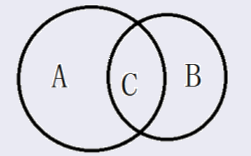
\includegraphics[height=50pt]{venn_0.png}
\end{center}
圆$A$表示擅长唱歌的,圆$B$表示擅长画画的,它们的相交区域$C$表示
既擅长唱歌也擅长画画的,容易算出答案是$a+b-c$。
\end{solution}

\end{frame}

\begin{frame}{总览}

\begin{block}{论文内容}
\begin{enumerate}
\item {\color<2>{red}{容斥原理——组合计数中的常用方法}}
\item {\color<2>{red}{例题——硬币购物(HAOI 2008)}}
\item {\color<2>{red}{例题——游戏}}
\item 容斥原理在数论和概率论中的推广
\item 容斥原理的一般化
\item 例题——有标号DAG计数
\end{enumerate}
\end{block}

\end{frame}

\begin{frame}{容斥原理}

设有限集合$U$,用$P_1,P_2$两种性质描述集合中的元素,设
满足$P_1$性质的元素组成集合$S_1$,满足$P_2$性质的元素组成集合$S_2$,
那么{\color{red}至少满足一个性质}的元素组成的集合可以用$S_1 \cup S_2$表示,
{\color{red}满足所有性质}的元素组成的集合可以用$S_1 \cap S_2$表示,则有:
\begin{eqnarray*}
|S_1 \cup S_2| = |S_1| + |S_2| - |S_1 \cap S_2|
\end{eqnarray*}
其中,$|S|$表示集合$S$中的元素个数。 \\

\end{frame}

\begin{frame}{容斥原理}

考虑用三种性质描述集合中的元素,类似地,我们利用文氏图分析,有:
\begin{center}
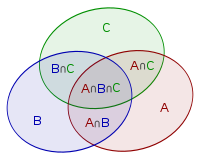
\includegraphics[height=100pt]{venn_1.png}
\end{center}
\begin{eqnarray*}
|S_1 \cup S_2 \cup S_3| & = & |S_1| + |S_2| + |S_3| - |S_1 \cap S_2| - |S_1 \cap S_3| - |S_2 \cap S_3| +{} \\
                        &   & {}+ |S_1 \cap S_2 \cap S_3|
\end{eqnarray*}

\end{frame}

\begin{frame}{容斥原理}

一般地,我们用$n$种性质$P_1,P_2,\cdots,P_n$描述集合$U$中的元素,且满足$P_i$性质的元素
组成集合$S_i$,那么

\begin{theorem}
至少满足$P_1,P_2,\cdots,P_n$中一个性质的元素的个数是:
\begin{eqnarray*}
|S_1 \cup S_2 \cup \cdots \cup S_n| & = & \sum_{i}{|S_i|} - \sum_{i<j}{|S_i \cap S_j|} + \sum_{i<j<k}{|S_i \cap S_j \cap S_k|} - \cdots{} \\
                                    &   & {}\cdots + (-1)^{n-1}{|S_1 \cap S_2 \cap \cdots S_n|}
\end{eqnarray*}
\end{theorem}

\end{frame}

\begin{frame}{容斥原理}

\begin{block}{一般方法}
\begin{enumerate}
\item 从{\color{red}集合}的角度分析问题;
\item 找出全集$U$和若干描述元素的性质$P_i$;
\item 利用容斥原理{\color{red}转化}和{\color{red}分解}问题,分别求解;
\item 合并答案。
\end{enumerate}
\end{block}

\pause

\begin{block}{时间复杂度}
一般来说,容斥原理的时间复杂度对于集合个数$n$是指数级的。 \\
但是,如果若干集合的交集的大小只与集合个数有关,就可以线性枚举集合的个数,通过组合数来计算。
\end{block}

\end{frame}

\begin{frame}{例题——硬币游戏(HAOI)}

\begin{problem}
有$4$种面值的硬币,第$i$种硬币的面值是$c_i$。有$n$次询问,每个询问中第$i$种硬币的数目是$d_i$,
以及一个购物款$s$,回答付款方法的数目。数据规模$n \le 10^3,s \le 10^5$。
\end{problem}

\pause

\begin{solution}
考虑一次询问,第$i$种硬币使用的数目是$x_i$,那么需要满足
\[
c_1x_1+c_2x_2+c_3x_3+c_4x_4=s\ \mbox{且}\ x_i \le d_i
\]
我们发现,这是一个经典的多重背包问题,但是动态规划是会超时的。
\end{solution}

\end{frame}

\begin{frame}{例题——硬币游戏(HAOI)}

\begin{solution}
我们进行一步{\color{red}补集转化},求至少一个$x_i$不满足条件的解的个数。 \par
令$S_i$表示满足$x_i \ge d_i+1$的解集,那么我们要求的就是$|S_1 \cup S_2 \cup S_3 \cup S_4|$,利用容斥原理可以把问题转化为求若干集合交集大小的问题。
\end{solution}

\pause

\begin{solution}
我们以$|S_1 \cap S_2|$为例。它要求$x_1 \ge d_1 + 1, x_2 \ge d_2 + 1$。 \par
\pause
我们令$y_1=x_1-(d_1+1)$,$y_2=x_2-(d_2+1)$,$y_3=x_3$,$y_4=x_4$,那么考虑
\[
s'=s-(d_1+1)-(d_2+1)
\]
我们的问题就变成了求$c_1y_1+c_2y_2+c_3y_3+c_4y_4=s'$的非负整数解数目,这个就是经典的无限背包问题了。 \par
\pause
我们只需要做一遍背包预处理$O(4m)$,$m$是询问中$s$的最大值,然后利用容斥原理就能做到每组询问$O(2^4)$。
\end{solution}

\end{frame}

\begin{frame}{例题——游戏}

\begin{problem}
\begin{itemize}
\item {\color<2>{red}Alice和Bob在玩游戏。}
\item {\color<3>{red}他们有一个$n$个点的无向完全图,设所有的边组成了集合$E$。}
\item {\color<4>{red}他们想取遍$E$的非空子集,对每个集合进行估价,$S$的估价记为$f(S)$。}
\item {\color<5>{red}考虑$n$个点与$S$中的边组成的图,用$m$种颜色对所有点染色。}
\item {\color<6>{red}同一个联通块的点必须染成一种颜色,$f(S)$等于这个图的染色方案数。}
\item {\color<7>{red}当$|S|$为奇数时,Alice的分值加上$f(S)$,否则Bob的分值加上$f(S)$。}
\item {\color<8>{red}求最后Alice的分值减去Bob的分值的值模$10^9+7$的结果。}
\item {\color<9>{red}数据规模$n,m \le 10^6$。时间限制$1$秒。}
\end{itemize}
\end{problem}

\end{frame}

\begin{frame}{例题——游戏}

例如,$n=3,m=2$,集合中只有一条边时,有如下四种染色方式:

\begin{center}
\begin{tabular}{c|c}
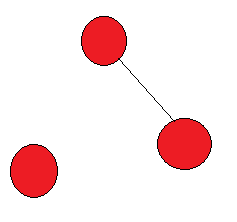
\includegraphics[height=70pt]{game_0.png} & 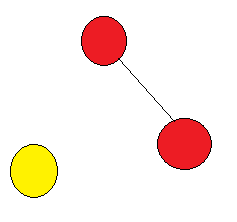
\includegraphics[height=70pt]{game_1.png} \\ \hline
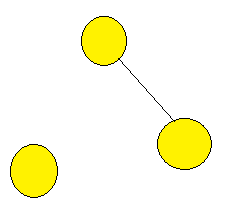
\includegraphics[height=70pt]{game_2.png} & 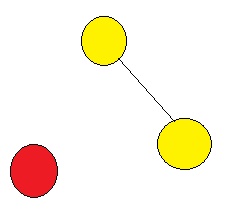
\includegraphics[height=70pt]{game_3.png} \\
\end{tabular}
\end{center}

\end{frame}

\begin{frame}{例题——游戏}

此题有一个强推式子的办法,如下图: \par
\begin{center}
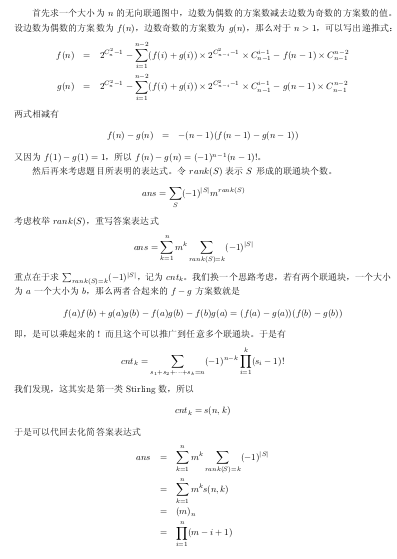
\includegraphics[height=170pt]{math.png}
\end{center}
\par
繁琐!

\end{frame}

\begin{frame}{例题——游戏}

\begin{block}{初步分析}
\begin{itemize}
\item 一方面,我们无法枚举边集$E$的所有子集;
\item 另一方面,对于边数相同的不同集合,图中的联通块数不一定一样。
\end{itemize}
当我们无法从表面寻找突破口时,应写出问题的数学形式,再进行分析。
\end{block}

\pause

\begin{block}{进一步分析}
\begin{center}
{\color{red}同一个联通块的点染成一种颜色} $\iff$ {\color{red}一条边连接的两个点染成一种颜色}
\end{center}
设$x_i$表示第$i$个点的颜色,则一条边$(i,j)$就表示一个条件$[x_i=x_j]$。令$F(C)$表示
,需要满足的条件组成的集合是$C$时,这个图的染色方案数。 \\
记Alice的得分为$scoreA$,Bob的得分为$scoreB$。
\end{block}

\end{frame}

\begin{frame}{例题——游戏}

\begin{block}{数学形式}
\begin{eqnarray*}
scoreA & = & \sum_{\varnothing \neq S \subseteq E,|S|\mbox{是奇数}} F\biggl([x_i = x_j] | (i,j) \in S\biggr) \\
scoreB & = & \sum_{\varnothing \neq S \subseteq E,|S|\mbox{是偶数}} F\biggl([x_i = x_j] | (i,j) \in S\biggr)
\end{eqnarray*}
\end{block}

\pause

\begin{block}{数学形式}
\begin{eqnarray*}
ans & = & \sum_{\emptyset \neq S \subseteq E} (-1)^{|S|-1} F\biggl([x_i = x_j] | (i,j) \in S\biggr)
\end{eqnarray*}
\end{block}

\end{frame}

\begin{frame}{例题——游戏}

\begin{block}{数学形式}
考虑$F\biggl([x_i=x_j] | (i,j) \in S\biggr)$的含义。 \\
满足$S$中所有边对应条件时,图的染色方案数。 \\
\end{block}

\pause

\begin{block}{数学形式}
令$T_e$表示满足$e$这条边对应条件,所有图的染色方案的集合。 \\
则$F\biggl([x_i=x_j] | (i,j) \in S\biggr)=|\bigcap_{e \in S} T_e|$。
\end{block}

\end{frame}

\begin{frame}{例题——游戏}

\begin{block}{数学形式}
设$E$的大小即总边数为$Q$,我们给边集$E$中所有的边从$1$到$Q$编号,则
\begin{eqnarray*}
ans & = & \sum_{|S|=1} F(S) - \sum_{|S|=2} F(S) + \cdots + (-1)^{Q-1} F(E) \\
    & = & \sum_{i}{|T_i|} - \sum_{i<j}{|T_i \cap T_j|} + \cdots + (-1)^{Q-1}{|T_1 \cap T_2 \cap \cdots \cap T_Q|}
\end{eqnarray*}
\pause
上式右边与容斥原理的形式相同,尝试{\color{red}逆向分析}出$ans$的含义,即
\pause
\begin{eqnarray*}
ans & = & |T_1 \cup T_2 \cup \cdots \cup T_Q|
\end{eqnarray*}
即{\color{red}至少一条边对应的条件满足}!
\end{block}

\end{frame}

\begin{frame}{例题——游戏}

\begin{solution}
我们问题变成了:$n$个点,$m$种颜色,至少两个点颜色相同,求染色方案数。 \\
进行一步{\color{red}补集转化},求点两两颜色不同的染色方案数,这个显然是
\[
m(m-1)(m-2)\cdots(m-n+1)
\]
所以答案就是
\[
m^n - \prod_{i = 1}^{n} (m - i + 1)
\]
\end{solution}

\end{frame}

\begin{frame}{例题——游戏}

\begin{block}{总结}
\begin{enumerate}
\item 写出问题的数学形式,用各种技巧化简;
\item {\color{red}逆向}使用容斥原理,分析答案表达式的真正含义;
\item 用一种可行的方式计算答案。
\end{enumerate}
\end{block}

\end{frame}

\begin{frame}{总结}

\begin{block}{思想}

\begin{enumerate}
\item {\color{red}隔离法}
\item {\color{red}整体法}

\pause

\item {\color{red} $\Rightarrow$ 转化!}
\end{enumerate}

\end{block}

\end{frame}

\begin{frame}{感谢}

\begin{itemize}
\item 感谢父母对我的养育
\item 感谢我的教练成都七中的张君亮老师,以及其他所有给予我支持的老师
\item 感谢罗雨屏、李凌霄、钟皓曦等同学的帮助
\item 感谢CCF给我一个展示自己的机会
\item 感谢各位的认真听讲
\end{itemize}

\end{frame}

\begin{frame}

\begin{center}
\Huge{欢迎大家批评指正!}
\end{center}

\end{frame}

\begin{frame}{容斥原理}

\begin{proof}
考虑一个元素$x$,它属于$m$个集合,我们重标号为$T_1,T_2,\cdots,T_m$,
那么因为上式右边我们计算的都是若干集合的交集,所以只用考虑这$m$个集合的组合,又因为这$m$个集合都
包含$x$,所以对于任意多个集合,它们的交集中都有$x$,只有计数的符号不同,即
\begin{eqnarray*}
cnt & = & \sum_{i}{1} - \sum_{i<j}{1} + \sum_{i<j<k}{1} - \cdots + (-1)^{m-1} \cdot 1 \\
    & = & C_m^1 - C_m^2 + C_m^3 - \cdots + (-1)^{m-1} C_m^m \\
    & = & C_m^0 - \left(C_m^0 - C_m^1 + C_m^2 - C_m^3 + \cdots + (-1)^m C_m^m\right) \\
	& = & 1 - (1-1)^m \\
	& = & 1
\end{eqnarray*}
其中$C_n^m$表示组合数,证明中结合了二项式定理。
\end{proof}

\end{frame}

\end{document}
